% =====================================================================
%  Why Johnny Can't Use Agents — Conference poster (ACM CAIS 2026)
%  48 in × 48 in (4 ft × 4 ft) square format
%  Compile with: xelatex poster.tex
% =====================================================================

\documentclass[final]{article}

\usepackage[paperwidth=48in,paperheight=48in,top=1in,bottom=1in,left=1in,right=1in]{geometry}

% ----- Fonts --------------------------------------------------------
\usepackage{fontspec}
\setmainfont{Source Serif 4}[
  UprightFont   = * ,
  ItalicFont    = * Italic ,
  BoldFont      = * SemiBold ,
  BoldItalicFont= * SemiBold Italic ,
  Ligatures     = TeX ,
  Numbers       = OldStyle ]
\newfontfamily\displayfont{Source Serif 4}[
  Numbers      = Lining ,
  Ligatures    = TeX ]
\newfontfamily\sansfont{Inter}[
  UprightFont  = * ,
  BoldFont     = * Bold ,
  Ligatures    = TeX ,
  Numbers      = Lining ]
\newfontfamily\monofont{Menlo}[Scale=0.92]
\newfontfamily\impactfont{Impact}

% ----- Colors -------------------------------------------------------
\usepackage{xcolor}
\definecolor{paper}{HTML}{E9F1E3}      % light Lacoste-green page background
\definecolor{paperTwo}{HTML}{DCEAD0}   % card fill (slightly deeper green)
\definecolor{paperThree}{HTML}{CDE0BE} % faint grid green
\definecolor{ink}{HTML}{1A1A1A}
\definecolor{inkSoft}{HTML}{3F4A40}
\definecolor{inkMuted}{HTML}{78836F}
\definecolor{crimson}{HTML}{1C5D3A}    % Lacoste green accent (was brick red)
\definecolor{blueAcc}{HTML}{2E5A88}
\definecolor{orcCol}{HTML}{2E5A88}   % Orchestration — blue   (matches paper)
\definecolor{creCol}{HTML}{4F7A52}   % Creation       — green  (matches paper)
\definecolor{insCol}{HTML}{C2474A}   % Insight        — red    (matches paper)
\definecolor{rulerCol}{HTML}{D9D2BD} % faint foot rulers
% Chart colors (match analysis script Mean-SUS-Scores-By-Task-And-Agent-with-CI)
\definecolor{opBar}{HTML}{E37569}   % coral — Operator
\definecolor{manusBar}{HTML}{5DAB94} % teal-green — Manus
% Bangor et al. (2009) SUS adjective bands — very pale (script uses alpha=0.6)
\definecolor{susWorst}{HTML}{FCE0DA}     % Worst Imaginable (0--25)
\definecolor{susPoor}{HTML}{FCEBD5}      % Poor             (25--50)
\definecolor{susOk}{HTML}{FCF5D6}        % OK               (50--65)
\definecolor{susGood}{HTML}{EAF2D2}      % Good             (65--80)
\definecolor{susExcellent}{HTML}{D9EAD3} % Excellent        (80--90)
\definecolor{susBest}{HTML}{DBEDF7}      % Best Imaginable  (90--100)

\pagecolor{paper}
\color{ink}

% ----- Packages -----------------------------------------------------
\usepackage{tikz}
\usetikzlibrary{positioning,calc,arrows.meta,shapes.geometric,backgrounds,fit,decorations.pathreplacing}
\usepackage{pgfplots}
\pgfplotsset{compat=1.18}
\usepackage{graphicx}
\usepackage{tcolorbox}
\tcbuselibrary{skins,breakable}
\usepackage{qrcode}
\usepackage{anyfontsize}
\usepackage{ragged2e}
\usepackage[autostyle=true]{csquotes}
\usepackage{microtype}

\pagestyle{empty}
\setlength{\parindent}{0pt}
\setlength{\parskip}{0pt}

% ----- Optional overlays --------------------------------------------
\newif\ifdraftgrid
\draftgridfalse  % flipped on by build.sh for diagnostic PDF
\newif\iffootrulers
\footrulerstrue  % faint 1-ft rulers always on (set false to remove)

% Macro that draws the overlays (called at end of document so they're on top)
\newcommand{\drawoverlays}{%
  \iffootrulers
    \begin{tikzpicture}[remember picture, overlay]
      \begin{scope}[shift={(current page.south west)}]
        \foreach \x in {1,2,3}{%
          \draw[rulerCol, line width=0.57pt] (\x*12in, 0) -- (\x*12in, 48in);
        }
        \foreach \y in {1,2,3}{%
          \draw[rulerCol, line width=0.57pt] (0, \y*12in) -- (48in, \y*12in);
        }
      \end{scope}
    \end{tikzpicture}%
  \fi
  \ifdraftgrid
    \begin{tikzpicture}[remember picture, overlay]
      \begin{scope}[shift={(current page.south west)}]
        \foreach \x in {0,1,...,4}{%
          \draw[crimson!80, line width=2.85pt, dash pattern=on 16pt off 12pt]
            (\x*12in, 0) -- (\x*12in, 48in);
        }
        \foreach \y in {0,1,...,4}{%
          \draw[crimson!80, line width=2.85pt, dash pattern=on 16pt off 12pt]
            (0, \y*12in) -- (48in, \y*12in);
        }
        \foreach \i [count=\ci] in {0,1,2,3}{%
          \foreach \j [count=\cj] in {3,2,1,0}{%
            \node[font=\sansfont\fontsize{136.8pt}{136.8pt}\selectfont\bfseries,
                  color=crimson!25, anchor=center]
                  at (\i*12in+6in, \j*12in+6in)
                  {\ifcase\ci A\or B\or C\or D\fi\cj};
          }
        }
        \foreach \x in {1,2,3}{%
          \node[font=\sansfont\fontsize{36.48pt}{41.04pt}\selectfont\bfseries,
                color=crimson, fill=paper, inner sep=4.56pt]
                at (\x*12in, 47.4in) {\x\,ft};
        }
        \foreach \y in {1,2,3}{%
          \node[font=\sansfont\fontsize{36.48pt}{41.04pt}\selectfont\bfseries,
                color=crimson, fill=paper, inner sep=4.56pt, rotate=90]
                at (0.6in, \y*12in) {\y\,ft};
        }
      \end{scope}
    \end{tikzpicture}%
  \fi}

% ----- Helpers ------------------------------------------------------
% Single heading per section — big crimson numbered title, no eyebrow, no rule
\newcommand{\sectionHead}[2]{%
  {\displayfont\fontsize{44pt}{50pt}\selectfont%
   \textcolor{crimson}{#1.\,}#2\par}}
\newcommand{\sectionHeadColored}[3]{%
  {\displayfont\fontsize{44pt}{50pt}\selectfont%
   \textcolor{#3}{#1.\,}#2\par}}

% Vertical gap between bands — no horizontal rule
\newcommand{\bandGap}{\par\vspace{42pt}}
\newcommand{\bandGapSmall}{\par\vspace{15.96pt}}
% Space after a section's big heading, before its content body.
\newcommand{\headPad}{\par\vspace{13.68pt}}

% =====================================================================
\begin{document}
\fontsize{29.64pt}{38.76pt}\selectfont

% ─────────────────────────────────────────────────────────────────────
%  HERO — title (1 line, bold, no period) + subtitle (title case)
%  Logos top-right; author row directly beneath subtitle.
% ─────────────────────────────────────────────────────────────────────

% ----- Combined header logos (CMU + potato + SPUD/Lab text) ---------
% All three elements share a common vertical center so they sit on one line.
% Uses absolute inch coordinates for clarity.
\newcommand{\cmulogoheight}{2.736in}
\newcommand{\headerLogos}{%
  \begin{tikzpicture}[baseline=(current bounding box.center)]
    \useasboundingbox (0in,0in) rectangle (13.984in, 2.736in);
    % CMU wordmark (left), 1.8in square.
    \node[anchor=south west, inner sep=0pt] at (0in, 0in)
      {
\includegraphics[height=2.736in]{assets/cmu-logo.png}};
    % Potato (middle), 1.8in square, with a healthy gap from CMU.
    \node[anchor=south west, inner sep=0pt] at (3.8in, 0in)
      {
\includegraphics[height=2.736in]{assets/spud-lab-potato.png}};
    % SPUD and Lab stacked at ~61pt (15 % smaller than the previous 72 pt) so the
    % stack sits ~85 % of the CMU height — the potato is now visibly taller than
    % the text. The text is also recentered vertically within the potato's
    % bounding box.
    \node[anchor=base west, inner sep=0pt] at (6.916in, 1.368in)
      {\impactfont\fontsize{92.72pt}{92.72pt}\selectfont\color{ink} SPUD};
    \node[anchor=base west, inner sep=0pt] at (6.916in, 0.304in)
      {\sansfont\fontsize{92.72pt}{95.76pt}\selectfont\color{inkSoft} Lab};
  \end{tikzpicture}%
}

% ----- Force-circular image clip (border-radius:50% for any PNG) ----
% Usage: \circphoto{path}{diameter-in-inches}
\newcommand{\circphoto}[2]{%
  \begin{tikzpicture}[x=1in,y=1in]
    \clip (0,0) circle ({#2/2});
    \node[inner sep=0pt] at (0,0) {\includegraphics[width=#2in,height=#2in]{#1}};
  \end{tikzpicture}%
}

% Hero: title (left) + combined logos block (right). The three logo elements
% — CMU, potato, SPUD/Lab text — all share one common vertical baseline.
% ----- Header: logos (left) | title (PAGE-CENTERED) | QR (right) -----
% Side blocks are equal width so the centre block sits at the true page centre;
% asymmetric content (wide logos vs. compact QR) is absorbed inside each side.
\noindent
\begin{minipage}[c]{11.5in}
  \scalebox{0.78}{\headerLogos}
\end{minipage}%
\begin{minipage}[c]{23in}\centering
  {\displayfont\fontsize{82pt}{86pt}\selectfont\bfseries
   Why Johnny \textcolor{crimson}{\textit{Can\textquoteright t}} Use Agents\par}
  \vspace{6pt}
  {\displayfont\fontsize{32pt}{39pt}\selectfont\itshape\color{inkSoft}
   Industry Aspirations Versus User Realities With AI Agents\par}
\end{minipage}%
\begin{minipage}[c]{11.5in}\raggedleft
  \begin{minipage}[t][2.13in][t]{6.7in}\raggedleft
    {\sansfont\fontsize{24pt}{30pt}\selectfont\color{crimson}\textbf{\textls[160]{READ THE PAPER}}}\vfill
    {\sansfont\fontsize{20pt}{25pt}\selectfont\color{inkSoft}doi.org/10.1145/3786335.3813140}\vfill
    {\sansfont\fontsize{18pt}{23pt}\selectfont\color{inkMuted}\textls[120]{\MakeUppercase{Funded by NSF Award} \#2316768}}\vfill
    {\sansfont\fontsize{18pt}{23pt}\selectfont\color{inkMuted}\textls[120]{CC BY 4.0}}
  \end{minipage}\hspace{0.32in}%
  \begin{minipage}[t][2.13in][c]{2.13in}
\includegraphics[width=2.13in,height=2.13in]{assets/cais-qr.png}\end{minipage}
\end{minipage}

\vspace{12pt}

% ----- Author row (centered) ---------------------------------------
\newcommand{\authorBlock}[3]{%
  \begin{minipage}[t]{5in}\centering
    \circphoto{#1}{2.28}\\[6.84pt]
    {\displayfont\fontsize{34.2pt}{38.76pt}\selectfont #2}\\[3.42pt]
    {\sansfont\fontsize{19.38pt}{22.8pt}\selectfont\color{inkMuted}\textls[140]{#3}}
  \end{minipage}%
}
\noindent
\begin{minipage}{\linewidth}\centering
  \authorBlock{assets/pradyumna-circle.png}{Pradyumna Shome}{Carnegie Mellon University}\hspace{0.7in}%
  \authorBlock{assets/sashreek-circle.png}{Sashreek Krishnan}{Carnegie Mellon University}\hspace{0.7in}%
  \authorBlock{assets/sauvik-circle.png}{Sauvik Das}{Carnegie Mellon University}%
\end{minipage}

\bandGap

% ─────────────────────────────────────────────────────────────────────
%  STATS STRIP — 4 headline numbers
% ─────────────────────────────────────────────────────────────────────
\noindent
\newcommand{\statBlock}[3]{%
  \begin{minipage}[t]{0.2\linewidth}\centering
    {\displayfont\fontsize{80pt}{80pt}\selectfont #1}\\[2.28pt]
    {\displayfont\fontsize{27.36pt}{34.2pt}\selectfont #2}\\[2.28pt]
    {\sansfont\fontsize{15.96pt}{20.52pt}\selectfont\color{inkMuted}\textls[200]{\MakeUppercase{#3}}}
  \end{minipage}}
\begin{minipage}{\linewidth}\centering
  \statBlock{102}{commercial AI agents reviewed}{Systematic review corpus}\hspace{0.9in}%
  \statBlock{31}{participants observed}{Think-aloud study}\hspace{0.9in}%
  \statBlock{5}{usability barriers identified}{Thematic analysis}\hspace{0.9in}%
  \statBlock{6}{design recommendations}{For agent builders}%
\end{minipage}

\bandGap

% ─────────────────────────────────────────────────────────────────────
%  RESEARCH QUESTIONS + STATE OF THE WORLD (compressed related work)
% ─────────────────────────────────────────────────────────────────────
\noindent
\begin{minipage}[t]{\linewidth}
  \begin{minipage}[t]{0.485\linewidth}
    \sectionHead{1}{The state of the world.}
    \headPad
    \newcommand{\sowBullet}[1]{%
      {\fontsize{34pt}{43pt}\selectfont\color{inkSoft}%
       \leftskip=0.6in
       \noindent\hskip-0.6in\makebox[0.6in][l]{\textcolor{crimson}{\textbullet}}#1\par}%
      \vspace{16pt}}
    \sowBullet{Industry benchmarks test whether agents \textit{can} complete tasks: \textbf{capability, not usability.}}
    \sowBullet{They sidestep the human side: \textbf{mental models, trust, oversight, recovery.}}
    \sowBullet{We bridge the gap: audit the marketed promise of \textbf{102 commercial agents,} then test whether real end-users can \textbf{realize} it on two leading agents.}
  \end{minipage}\hfill
  \begin{minipage}[t]{0.485\linewidth}
    \sectionHead{2}{The research questions.}
    \headPad
    \noindent
    \begin{minipage}[t]{\linewidth}
      \tcbox[colback=paperTwo,colframe=ink,boxrule=1.14pt,sharp corners,
             boxsep=0pt,left=25.08pt,right=25.08pt,top=20.52pt,bottom=20.52pt,
             width=\linewidth,valign=top,nobeforeafter]{%
        \begin{minipage}[t]{\dimexpr\linewidth-58pt\relax}\raggedright
          {\sansfont\fontsize{22.8pt}{27.36pt}\selectfont\color{crimson}\textls[220]{\textbf{RQ1\,\,\,INDUSTRY}}}\par
          \vspace{6.84pt}
          {\displayfont\fontsize{34.2pt}{43.32pt}\selectfont
           How does the tech industry conceive of and market \textquotedblleft AI agents\textquotedblright?\par}
        \end{minipage}}\par
      \vspace{15.96pt}
      \tcbox[colback=paperTwo,colframe=ink,boxrule=1.14pt,sharp corners,
             boxsep=0pt,left=25.08pt,right=25.08pt,top=20.52pt,bottom=20.52pt,
             width=\linewidth,valign=top,nobeforeafter]{%
        \begin{minipage}[t]{\dimexpr\linewidth-58pt\relax}\raggedright
          {\sansfont\fontsize{22.8pt}{27.36pt}\selectfont\color{blueAcc}\textls[220]{\textbf{RQ2\,\,\,USERS}}}\par
          \vspace{6.84pt}
          {\displayfont\fontsize{34.2pt}{43.32pt}\selectfont
           What challenges do end-users face when using commercial AI agents for their advertised uses?\par}
        \end{minipage}}\par
    \end{minipage}
  \end{minipage}
\end{minipage}

\bandGap

% ─────────────────────────────────────────────────────────────────────
%  THREE-COLUMN PANEL — SELLS | EVALUATED | GOT
% ─────────────────────────────────────────────────────────────────────
\noindent
\begin{minipage}[t]{\linewidth}
  % ============================================================ COL 1
  \begin{minipage}[t]{0.315\linewidth}
    \sectionHead{3}{What the industry sells.}
    \vspace{9.12pt}
    {\fontsize{34pt}{43pt}\selectfont\color{inkSoft}
     102 marketed-as-agentic products cluster into three umbrella use cases. \textit{Categories overlap.}\par}
    \vspace{22.8pt}

    % Each umbrella row gets a fixed-height \parbox; content is top-aligned and
    % the empty tail of the box is always the same, so the visible gap between
    % Orchestration / Creation / Insight is uniform regardless of how the
    % description / "e.g." line happens to wrap.
    \newcommand{\taxRowHeight}{2.9in}
    \newcommand{\taxRow}[5]{%
      \noindent\parbox[t][\taxRowHeight][t]{\linewidth}{%
        \begin{minipage}[t]{0.64\linewidth}\raggedright
          {\displayfont\fontsize{48pt}{52pt}\selectfont\color{#1} #2}\\[9.12pt]
          {\fontsize{34pt}{43pt}\selectfont\color{inkSoft} #3}\\[6.84pt]
          {\fontsize{28pt}{34pt}\selectfont\itshape\color{inkMuted} e.g.\ #4}
        \end{minipage}\hfill
        \begin{minipage}[t]{0.32\linewidth}\raggedleft
          \vspace{0.2052in}
          \begin{tikzpicture}[baseline=-1.5ex]
            \fill[#1] (0,0) rectangle (#5*0.07,0.7);
          \end{tikzpicture}\\[4.56pt]
          {\displayfont\fontsize{95.76pt}{95.76pt}\selectfont\color{#1} #5}
        \end{minipage}%
      }\par}

    \taxRow{orcCol}{Orchestration}{Act on behalf of users in software interfaces: GUIs, automation.}{Agentforce, Copilot}{31}
    \taxRow{creCol}{Creation}{Generate structured artifacts: slides, websites, apps, docs.}{Lovable, Gamma, Beautiful.AI}{33}
    \taxRow{insCol}{Insight}{Distill large information sets into structured user-facing takeaways.}{Perplexity, Spotify AI DJ}{87}
    \vspace{4pt}
  \end{minipage}\hfill
  % ============================================================ COL 2
  \begin{minipage}[t]{0.315\linewidth}
    \sectionHead{4}{How we investigated it.}
    \vspace{9.12pt}
    {\fontsize{34pt}{43pt}\selectfont\color{inkSoft}
     We tested whether participants could realize the marketed promise on two leading commercial agents.\par}
    \vspace{22.8pt}

    \centering
    % Pipeline — boxes spaced wider so text isn't truncated by neighbour boxes.
    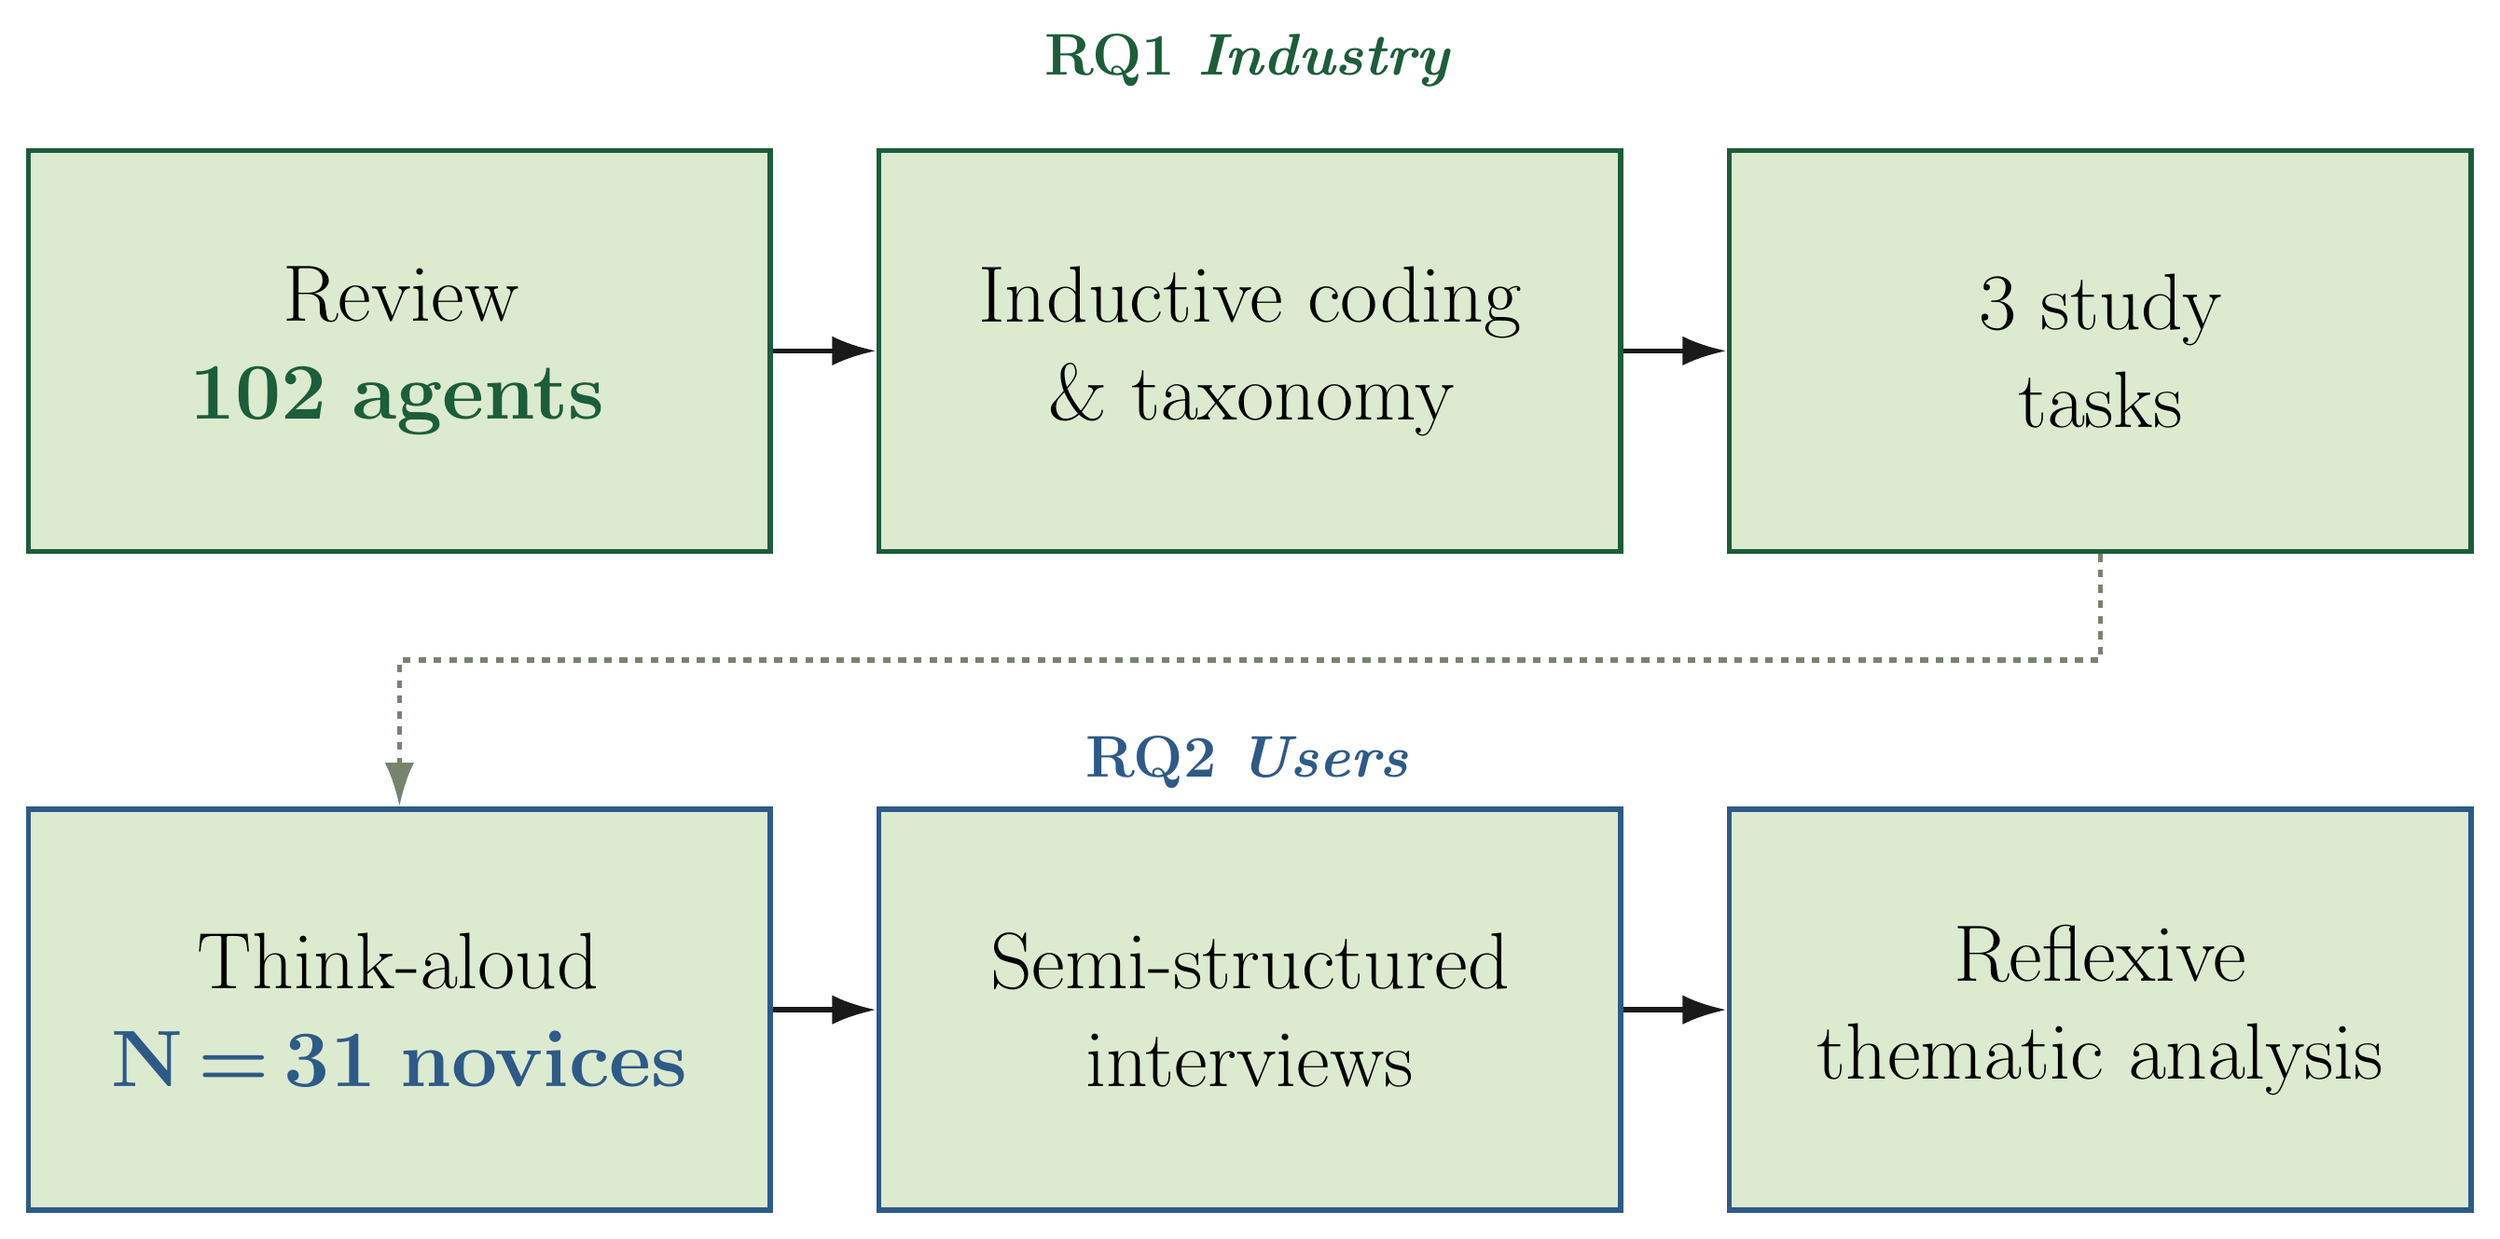
\begin{tikzpicture}[x=1.14in,y=1.14in,
        rqstep/.style={draw=crimson, line width=2.052pt, fill=paperTwo,
          inner sep=13.68pt, minimum height=2.15in, text width=3.6in,
          font=\displayfont\fontsize{31pt}{38pt}\selectfont, align=center},
        rq2step/.style={draw=blueAcc, line width=2.052pt, fill=paperTwo,
          inner sep=13.68pt, minimum height=2.15in, text width=3.6in,
          font=\displayfont\fontsize{31pt}{38pt}\selectfont, align=center},
        arr/.style={-{Latex[length=6mm,width=4mm]}, ink, line width=2.052pt},
      ]
      % RQ1 row — boxes at -3.6 / 0 / +3.6 (2.6in box + ~0.3in padding = 2.9in;
      % center-to-center spacing 3.6in leaves ~0.7in arrow length).
      \node[font=\sansfont\fontsize{22.8pt}{27.36pt}\selectfont\color{crimson}\bfseries,
            anchor=south] (rq1l) at (0,1.2) {RQ1\,\,\textit{Industry}};
      \node[rqstep, anchor=center] (rq1a) at (-4.0,0.0)
        {Review\\\textcolor{crimson}{\bfseries 102 agents}};
      \node[rqstep, anchor=center] (rq1b) at ( 0.0,0.0)
        {Inductive coding\\\&\ taxonomy};
      \node[rqstep, anchor=center] (rq1c) at ( 4.0,0.0)
        {3 study\\tasks};
      \draw[arr] (rq1a) -- (rq1b);
      \draw[arr] (rq1b) -- (rq1c);

      % RQ2 row
      \node[font=\sansfont\fontsize{22.8pt}{27.36pt}\selectfont\color{blueAcc}\bfseries,
            anchor=south] (rq2l) at (0,-2.1) {RQ2\,\,\textit{Users}};
      \node[rq2step, anchor=center] (rq2a) at (-4.0,-3.1)
        {Think-aloud\\\textcolor{blueAcc}{\bfseries N\,=\,31 novices}};
      \node[rq2step, anchor=center] (rq2b) at ( 0.0,-3.1)
        {Semi-structured\\interviews};
      \node[rq2step, anchor=center] (rq2c) at ( 4.0,-3.1)
        {Reflexive\\thematic analysis};
      \draw[arr] (rq2a) -- (rq2b);
      \draw[arr] (rq2b) -- (rq2c);
      \draw[arr,dashed,inkMuted] (rq1c.south) -- ++(0,-0.5) -| (rq2a.north);
    \end{tikzpicture}\par
    \vspace{13.68pt}
    {\monofont\fontsize{30pt}{36pt}\selectfont\color{crimson}\textls[180]{\MakeUppercase{Fig. 1}}\hspace{15.96pt}}%
    {\fontsize{34pt}{42pt}\selectfont\itshape\color{inkMuted}Mixed-methods pipeline. RQ1 builds the taxonomy; RQ2 tests whether real users realize it. User study approved by Carnegie Mellon University IRB.}
  \end{minipage}\hfill
  % ============================================================ COL 3
  \begin{minipage}[t]{0.315\linewidth}
    \sectionHead{5}{Quantitative measurements.}
    \vspace{9.12pt}
    {\fontsize{34pt}{43pt}\selectfont\color{inkSoft}
     Two commercial agents, \textcolor{crimson}{\textbf{Operator}} \&\ \textcolor{blueAcc}{\textbf{Manus}}, rated by participants using the System Usability Scale (\textit{SUS}, 0--100).\par}
    \vspace{22.8pt}

    \centering
    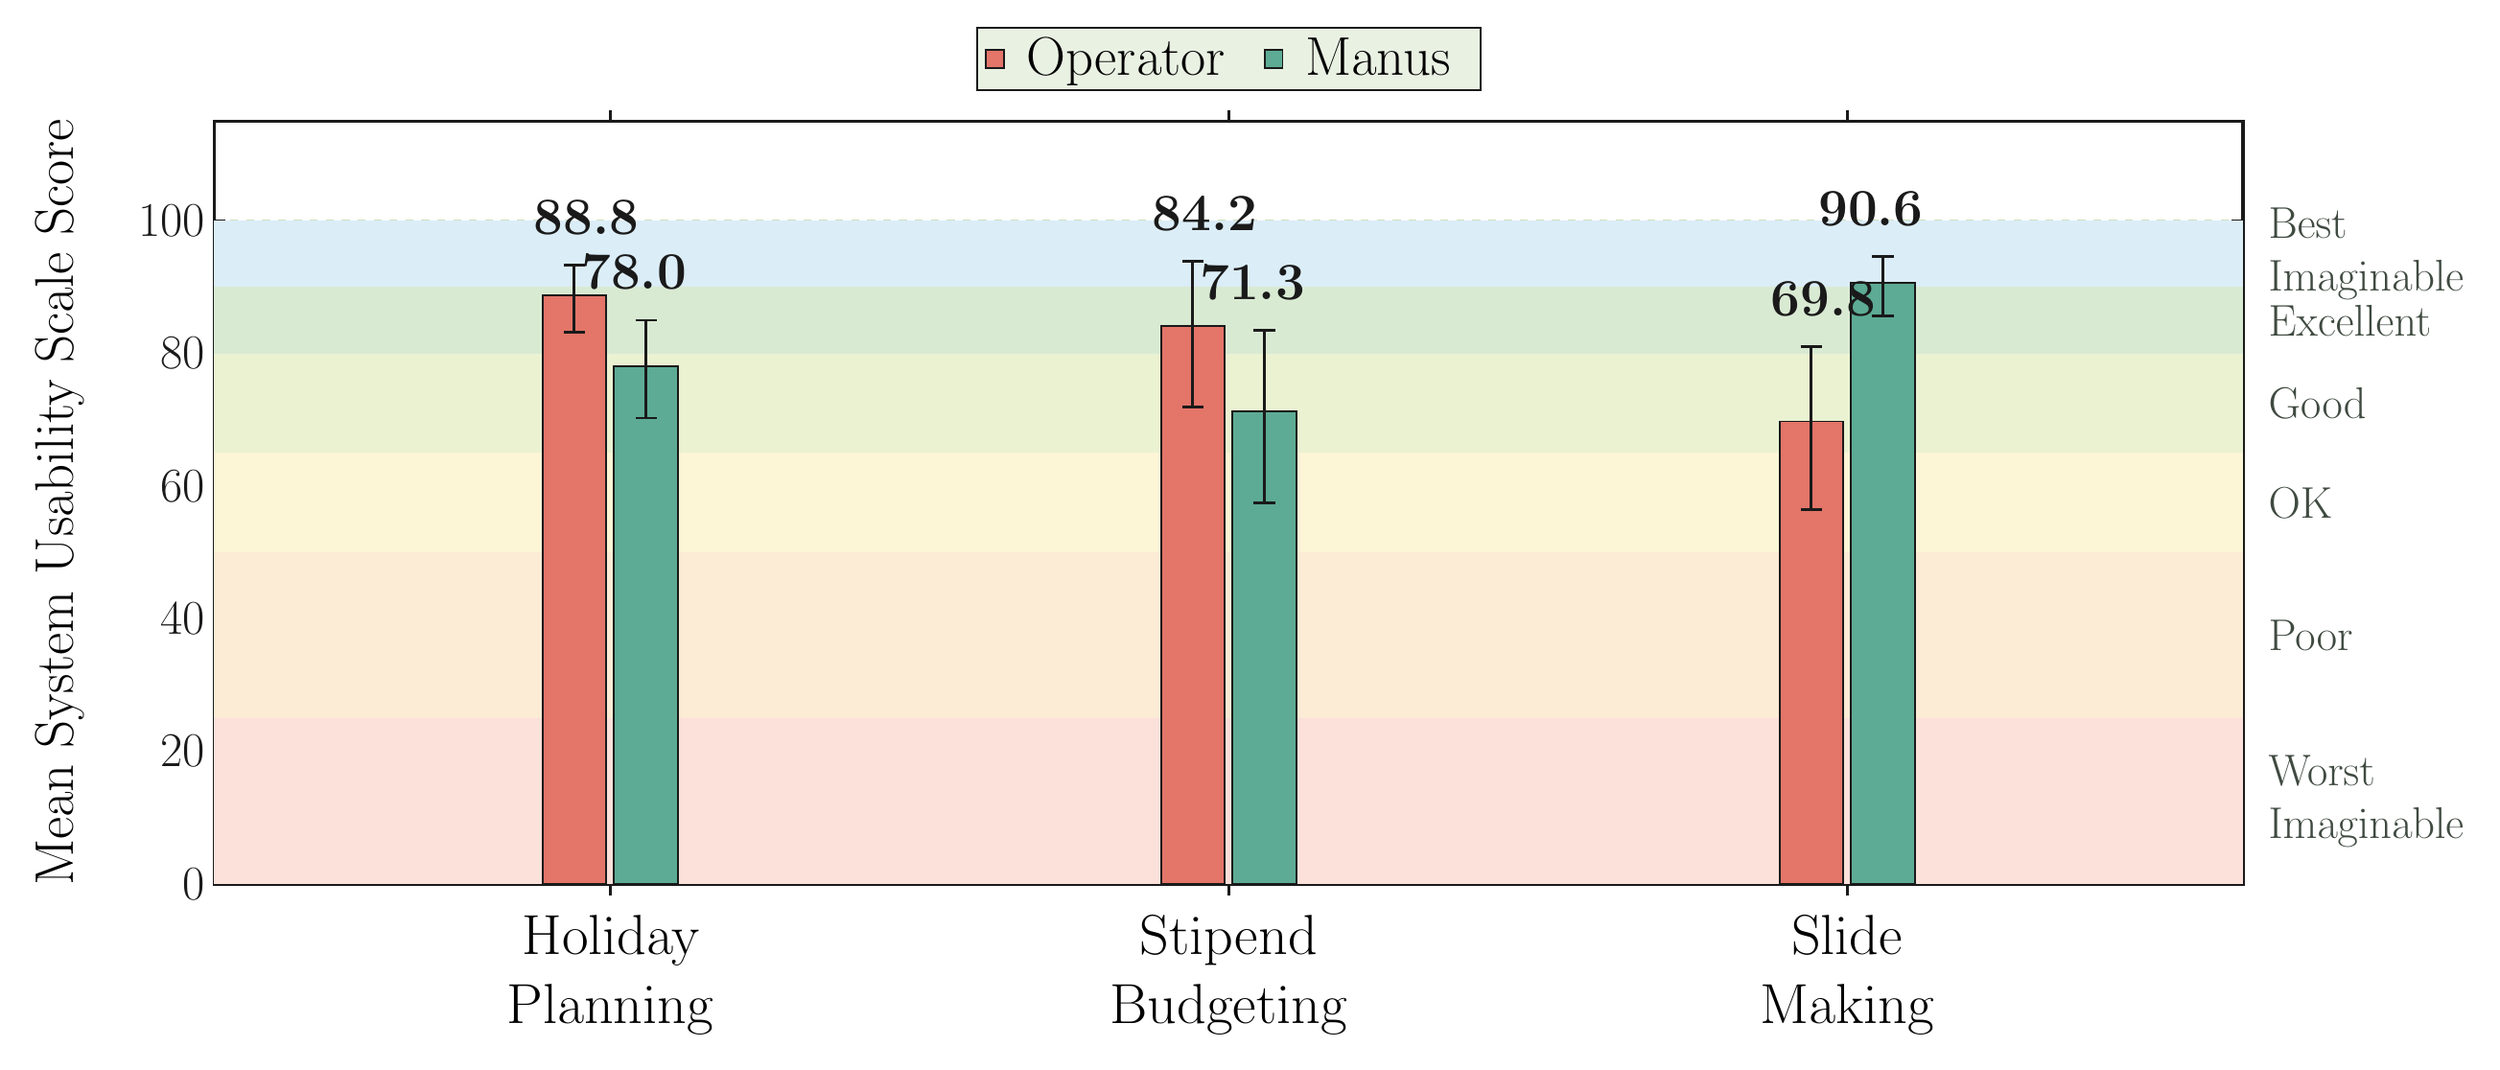
\begin{tikzpicture}
      \begin{axis}[
        ybar=3pt,
        bar width=24pt,
        width=11.2in,
        height=4.6in,
        ymin=0, ymax=115,
        ytick={0,20,40,60,80,100},
        ymajorgrids=true,
        major grid style={paperThree, line width=0.684pt, dashed},
        axis line style={ink, line width=1.14pt},
        tick style={ink, line width=1.14pt},
        symbolic x coords={H,St,Sl},
        xtick=data,
        xticklabels={
          {Holiday\\Planning},
          {Stipend\\Budgeting},
          {Slide\\Making}
        },
        xticklabel style={align=center, text width=3.69663in, yshift=-4pt,
          font=\displayfont\fontsize{21.28pt}{25.84pt}\selectfont},
        y tick label style={font=\sansfont\fontsize{18.24pt}{22.8pt}\selectfont\color{ink}},
        ylabel={\sansfont\fontsize{20.52pt}{25.08pt}\selectfont Mean System Usability Scale Score},
        ylabel style={yshift=13.68pt},
        legend style={
          font=\sansfont\fontsize{20.52pt}{25.08pt}\selectfont,
          at={(0.5,1.04)}, anchor=south, legend columns=-1,
          draw=ink, line width=0.684pt, fill=paper},
        /pgfplots/legend image code/.code={%
          \draw[#1, draw=ink, line width=0.684pt] (0cm,-0.12cm) rectangle (0.24cm,0.12cm);
        },
        enlarge x limits=0.32,
        clip=false,
        axis on top=false,
      ]
        % Six Bangor et al. SUS interpretation bands (very pale).
        \fill[susWorst,     draw=none] ({rel axis cs:0,0} |- {axis cs:H,0})  rectangle ({rel axis cs:1,0} |- {axis cs:H,25});
        \fill[susPoor,      draw=none] ({rel axis cs:0,0} |- {axis cs:H,25}) rectangle ({rel axis cs:1,0} |- {axis cs:H,50});
        \fill[susOk,        draw=none] ({rel axis cs:0,0} |- {axis cs:H,50}) rectangle ({rel axis cs:1,0} |- {axis cs:H,65});
        \fill[susGood,      draw=none] ({rel axis cs:0,0} |- {axis cs:H,65}) rectangle ({rel axis cs:1,0} |- {axis cs:H,80});
        \fill[susExcellent, draw=none] ({rel axis cs:0,0} |- {axis cs:H,80}) rectangle ({rel axis cs:1,0} |- {axis cs:H,90});
        \fill[susBest,      draw=none] ({rel axis cs:0,0} |- {axis cs:H,90}) rectangle ({rel axis cs:1,0} |- {axis cs:H,100});

        % Operator (coral) bars + asymmetric 95% bootstrap CI error bars.
        % Means and CI bounds are taken verbatim from
        % ai-agents-qualtrics-analysis/sus_summary_stats.csv.
        \addplot+[ybar, fill=opBar, draw=ink, line width=0.684pt,
            error bars/.cd, y dir=both, y explicit,
            error bar style={ink, line width=1.064pt},
            error mark options={rotate=90, ink, line width=1.064pt, mark size=4pt}]
          table[col sep=comma, row sep=\\, x=task, y=mean,
                y error plus=eplus, y error minus=eminus] {%
task,mean,eplus,eminus\\
H,88.75,4.50,5.50\\
St,84.17,9.72,12.23\\
Sl,69.75,11.25,13.25\\
          };
        \addlegendentry{\,\,Operator\,\,\,\,}
        % Manus (teal-green) bars + asymmetric CI error bars.
        \addplot+[ybar, fill=manusBar, draw=ink, line width=0.684pt,
            error bars/.cd, y dir=both, y explicit,
            error bar style={ink, line width=1.064pt},
            error mark options={rotate=90, ink, line width=1.064pt, mark size=4pt}]
          table[col sep=comma, row sep=\\, x=task, y=mean,
                y error plus=eplus, y error minus=eminus] {%
task,mean,eplus,eminus\\
H,78.00,7.00,7.75\\
St,71.25,12.25,13.75\\
Sl,90.58,4.04,5.00\\
          };
        \addlegendentry{\,\,Manus\,\,}

        % Six SUS-band labels on the right edge (vertical centers of each band).
        \def\suslab#1#2{%
          \node[anchor=west, xshift=6.08pt, align=left,
                font=\sansfont\fontsize{16.72pt}{19.76pt}\selectfont\color{inkSoft}]
            at ({rel axis cs:1,0} |- {axis cs:H,#1}) {#2};}
        \suslab{95}{Best\\Imaginable}
        \suslab{85}{Excellent}
        \suslab{72.5}{Good}
        \suslab{57.5}{OK}
        \suslab{37.5}{Poor}
        \suslab{12.5}{Worst\\Imaginable}

        % Bold mean-value labels above the error bars (no overlap).
        % x offset (±9pt) places the label centered above each bar; y =
        % mean + SD + 4 keeps the number clear of the upper error cap.
        \def\barlab#1#2#3#4{%
          \node[anchor=south, xshift=#1, yshift=3.04pt,
                font=\displayfont\fontsize{19.76pt}{21.28pt}\selectfont\bfseries\color{ink}]
            at (axis cs:#2,#3) {#4};}
        % y positions = mean + upper CI offset + 2 (clear of the upper cap).
        \barlab{-9pt}{H}{95.25}{88.8}    % Operator Holiday  88.75 + 4.50
        \barlab{+9pt}{H}{87.00}{78.0}    % Manus Holiday     78.00 + 7.00
        \barlab{-9pt}{St}{95.89}{84.2}   % Operator Stipend  84.17 + 9.72
        \barlab{+9pt}{St}{85.50}{71.3}   % Manus Stipend     71.25 + 12.25
        \barlab{-9pt}{Sl}{83.00}{69.8}   % Operator Slide    69.75 + 11.25
        \barlab{+9pt}{Sl}{96.62}{90.6}   % Manus Slide       90.58 + 4.04
      \end{axis}
    \end{tikzpicture}\par
    \vspace{9.12pt}
    {\monofont\fontsize{30pt}{36pt}\selectfont\color{crimson}\textls[180]{\MakeUppercase{Fig. 2}}\hspace{15.96pt}}%
    {\fontsize{34pt}{42pt}\selectfont\itshape\color{inkMuted}Mean SUS by task and agent. $n=9$--$13$ per cell. Error bars show 95\%\ bootstrap CIs of the mean. Bands are Bangor et al.\ adjective ratings.}\par
    \vspace{18.24pt}
    \tcbox[colback=ink,colframe=ink,sharp corners,boxsep=0pt,
           left=20.52pt,right=20.52pt,top=13.68pt,bottom=13.68pt,width=\linewidth]{%
      \begin{minipage}[t]{\dimexpr\linewidth-58pt\relax}\raggedright\color{paper}
        {\sansfont\fontsize{17.1pt}{21.66pt}\selectfont\color{paperTwo}\textls[220]{\textbf{THE SUS PARADOX}}}\par\vspace{3.42pt}
        {\displayfont\fontsize{27.36pt}{34.2pt}\selectfont\itshape
         Excellent SUS scores, yet five critical usability barriers persist beneath them.\par}
      \end{minipage}}
  \end{minipage}
\end{minipage}

\bandGap

% ─────────────────────────────────────────────────────────────────────
%  FIVE BARRIERS — single heading, no eyebrow
% ─────────────────────────────────────────────────────────────────────
\noindent
\begin{minipage}[t]{\linewidth}
  \sectionHead{7}{Five barriers to agent delegation.}
  \vspace{18.24pt}

  % Optional first arg = card height (row 2 cards carry less text, so are shorter).
  \newcommand{\barrierCard}[5][4.35in]{%
    \tcbox[colback=paperTwo,colframe=ink,boxrule=1.14pt,sharp corners,boxsep=0pt,
           left=27pt,right=27pt,top=24pt,bottom=24pt,
           width=\linewidth,height=#1,valign=top,nobeforeafter]{%
      \begin{minipage}[t]{\dimexpr\linewidth-58pt\relax}\raggedright
        {\displayfont\fontsize{40pt}{47pt}\selectfont \textcolor{crimson}{#2.\,}#3\par}
        \vspace{15pt}
        {\fontsize{34pt}{43pt}\selectfont\color{inkSoft} #4\par}
        \vspace{15pt}
        {\displayfont\fontsize{34pt}{44pt}\selectfont\itshape\color{ink}
         \textcolor{crimson}{\textbf{\textquotedblleft}}#5\textcolor{crimson}{\textbf{\textquotedblright}}\par}
      \end{minipage}}}

  % Row 1 — three cards.
  \noindent
  \begin{minipage}[t]{0.325\linewidth}
    \barrierCard{1}{Misaligned mental models}{Users can\textquoteright t predict capabilities, turning delegation into frustrating \textquotedblleft prompt gambling.\textquotedblright}{You\textquoteright ve got to sit there and make sure that your initial prompt is perfect.}
  \end{minipage}\hfill
  \begin{minipage}[t]{0.325\linewidth}
    \barrierCard{2}{Presuming trust}{Agents expect immediate delegation without first establishing credibility or competence signals.}{I was waiting for it to ask me for some more information.}
  \end{minipage}\hfill
  \begin{minipage}[t]{0.325\linewidth}
    \barrierCard{3}{Inflexible collaboration}{Agents act as \textquotedblleft lone-wolf\textquotedblright\ tools that fail to adapt to a user\textquoteright s need for hands-on oversight.}{It\textquoteright s kind of like I\textquoteright m giving you a job, and you\textquoteright re throwing the job back at me.}
  \end{minipage}

  \vspace{20pt}

  % Row 2 — two wider cards.
  \noindent
  \begin{minipage}[t]{0.494\linewidth}
    \barrierCard[3.0in]{4}{Communication overhead}{Excessive output and demand for articulation of complex, subjective preferences.}{Oh, my God! It threw out so much stuff\ldots\ it\textquoteright s almost overwhelming.}
  \end{minipage}\hfill
  \begin{minipage}[t]{0.494\linewidth}
    \barrierCard[3.0in]{5}{Metacognitive gaps}{Agents lack self-awareness of errors, leading to time-wasting \textquotedblleft try-fail cycles.\textquotedblright}{It just was kind of circling\ldots\ seeking to provide an answer rather than to say \textquotedblleft I don\textquoteright t know.\textquotedblright}
  \end{minipage}
\end{minipage}

\bandGap

% ─────────────────────────────────────────────────────────────────────
%  SIX RECOMMENDATIONS — 6-column row, taller cards so nothing squishes
% ─────────────────────────────────────────────────────────────────────
\noindent
\begin{minipage}[t]{\linewidth}
  \sectionHead{8}{Six design recommendations for building usable next-generation agents.}
  \vspace{18.24pt}

  \newcommand{\recCard}[4]{%
    \tcbox[colback=paperTwo,colframe=ink,boxrule=1.14pt,sharp corners,boxsep=0pt,
           left=24pt,right=24pt,top=21pt,bottom=21pt,
           width=\linewidth,height=2.85in,valign=top,nobeforeafter]{%
      \begin{minipage}[t]{\dimexpr\linewidth-58pt\relax}\raggedright
        {\displayfont\fontsize{40pt}{47pt}\selectfont \textcolor{crimson}{#1.\,}#3\par}
        \vspace{14pt}
        {\fontsize{34pt}{43pt}\selectfont\color{inkSoft} #4\par}
      \end{minipage}}}

  % Row 1
  \noindent
  \begin{minipage}[t]{0.325\linewidth}\recCard{1}{Delegation}{Know your user.}{Elicit preferences, skills, and collaboration styles before executing.}\end{minipage}\hfill
  \begin{minipage}[t]{0.325\linewidth}\recCard{2}{Metacognition}{Know yourself.}{Recognise capability limits, stop confidently, surface uncertainty.}\end{minipage}\hfill
  \begin{minipage}[t]{0.325\linewidth}\recCard{3}{Collaboration}{Be adaptable.}{Adapt to task type, confusion signals, and the user\textquoteright s control preference.}\end{minipage}

  \vspace{20pt}

  % Row 2
  \noindent
  \begin{minipage}[t]{0.325\linewidth}\recCard{4}{Oversight}{Measure twice, cut once.}{Surface planning artifacts and mid-task checkpoints to steer before failure.}\end{minipage}\hfill
  \begin{minipage}[t]{0.325\linewidth}\recCard{5}{Input}{Show, don\textquoteright t tell.}{Support modalities beyond text: examples, sketches, direct selection.}\end{minipage}\hfill
  \begin{minipage}[t]{0.325\linewidth}\recCard{6}{Iteration}{Next time\textquoteright s the charm.}{Enable precise contextual iteration, not new prompts that regress elsewhere.}\end{minipage}
\end{minipage}

\bandGap

% ─────────────────────────────────────────────────────────────────────
%  SECTION 9 — THREE SOCIOTECHNICAL AXES (implications for evaluation)
%  These are NOT axes we measured; they are axes we propose for future
%  evaluation of agentic systems. Titles + sub-bullets from slide 17.
% ─────────────────────────────────────────────────────────────────────
\noindent
\begin{minipage}[t]{\linewidth}
  \sectionHead{9}{Three sociotechnical axes for evaluating agentic systems.}
  \vspace{22.8pt}

  \newcommand{\axisCard}[5]{%
    \tcbox[colback=paperTwo,colframe=#1,boxrule=2.052pt,sharp corners,
           boxsep=0pt,left=25.08pt,right=25.08pt,top=22pt,bottom=22pt,
           width=\linewidth,height=2.55in,valign=top,nobeforeafter]{%
      \begin{minipage}[t]{\dimexpr\linewidth-58pt\relax}\raggedright
        {\displayfont\fontsize{38.76pt}{45.6pt}\selectfont \textcolor{crimson}{#2.\,}#3\par}
        \vspace{12pt}
        {\fontsize{34pt}{42pt}\selectfont\color{inkSoft} #4\par}
      \end{minipage}}}

  \noindent
  \begin{minipage}[t]{0.325\linewidth}
    \axisCard{insCol}{1}{Failure recovery.}
      {Intervention frequency, recovery time, and stall rate when stuck.}{}
  \end{minipage}\hfill
  \begin{minipage}[t]{0.325\linewidth}
    \axisCard{creCol}{2}{Authorship control.}
      {Plan adherence, precise-edit accuracy, and mid-task checkpoints.}{}
  \end{minipage}\hfill
  \begin{minipage}[t]{0.325\linewidth}
    \axisCard{orcCol}{3}{Trusted delegation.}
      {Credential management and least-privilege, observable handoffs.}{}
  \end{minipage}
\end{minipage}


\drawoverlays

\end{document}
